\documentclass[a4paper,12pt]{article}
    
    \usepackage[utf8]{inputenc}
    \usepackage[T1]{fontenc} 
    \usepackage[francais]{babel}
    \usepackage{amsmath}
    \usepackage{amssymb}
    \usepackage{graphicx}
    \usepackage{color}
    \usepackage{hyperref}
    \usepackage[left=2cm,right=2cm,top=2cm,bottom=2cm]{geometry}
    \usepackage{mathrsfs}
    \title{Application de chiffrement homomorphe a l'apprentissage automatique}

\author{BENISSA Sami\quad:\quad Université Paris 8}


\date{8 septembre 2017}
\begin{document}
\maketitle
\newpage
%\newpage
\renewcommand{\chaptername}{}
%\renewcommand{\contentsname}{sommaires}
\tableofcontents

\newpage
\section*{Remerciements}
\newpage
%\part{Partie 1}
\section{Présentation de l’entreprise}
\href{http://jolibrain.com/}{Jolibrain} est une jeune entreprise inovante et toulousaine dont le noyau est constitué de ``vétérans'' de l'Intelligence Articielle (IA) et du Web et d'autour duquel gravite un réseau d'experts.
Jolibrain a à coeur d'apporter des solutions efficaces à des problèmes concrets.

Jolibrain met au point des logiciels haute performance incluant les dernières avancées en matière d'IA. Les logiciels Jolibrain sont utilisés aussi bien chez de grands groupes que par des start up. Jolibrain regroupe en son sein l'expertise en  Machine Learning, Deep Learning, Reinforcement Learning, Stochastic Optimization, Search Enginesengin de recherche, system P2P et encore plus.

Jolibrain est fondé sur le logiciel libre. Les valeurs véhiculée par Jolibrain sont la créativité, la collaboration, le  partage et l'apprentissage. La majorité de la production est disponible publiquement et Open Source.

Les projet et produits de Jolibrain sont les suivants :
\begin{itemize}
\item   Service en Deep Learning :
  Jolibrain sont les auteurs de l'API  et du serveurOpen Source Deeplearning \href{https://github.com/beniz/deepdetect}{Deep Detect}.
\item Art: l'exposition Regognition de la Tate Gallery à Londre utilise un code Jolibrain.
\item
Cyber-securité: de grands groupes utilisent du code jolibrain pour la détection de malware et d'anomalies dans leurs logs.
\item
Contenu et médias: De grand groupes aussi bien que des start uop utilise des produits Jolibrain pour le filtrage et la modération de contenu.
\item
Images et recherche : Certains e-shopsmarchands en ligne mais aussi des agence spatiale utilisent jolibrain and aerospace agencies search and recommend visual elements running our pipeline pour la recherche et la recommandation.
\item
High tech et hardware : certaines start up du Deep Learning utilise le code Jolibrain pour leurs services cloud.
\end{itemize}

\newpage
\section{Introduction}
\subsection{Contexte : Big data et intelligence artificielle (IA)}
\subsection{Problématique : éthique et confidentialité}
\subsection{Objectif du stage}
Le But de  stage était de concevoir une application d'apprentissage automatique a partir des données chiffrées en utilisant un schéma de chiffrement homomorphe.\newline
Ce type d'application peut servir dans les domaines ou on veut appliquer de calcul sur des données privées.\newline
Par exemple chaque jour on voit sortir des applications d'apprentissage automatique dans le domaine médical mais la question est qu'on peut fournir le meme servir en gardant la confidentialité sur les informations des patients.\newline
La prémière étape durant la periode de stage l'objectif c'était de faire l'Etat de l'art sur les différents cryptosystème de chiffrerment homomorphe et de bien comprendre le concept de machine learning.\newline
La deuxième étape le but c'était d'implementer des algorithmes de machine learning sur des données clair afin de concevoir un modèle et régarder les différents métriques qu'il faut prendre en compte pour analyser l'efficacité du modèle.\newline
La dernière étape c'était pour implementer les memes algoritmes sur des données chiffrées et d'evaluer la différence par rapport au résultat obtenu au partir des algorithmes implementer dans la deuxième partie.\newline
\section{Etat de l'art} 
\subsection{Cryptographie}
\subsubsection{Chiffrement partiellement homomorphe}
\textit{definition : } On dit qu'un cryptosystème est partiellement homomorphe  s'il possède certaines caractéristiques algébriques qui le font commuter avec une opération mathématique, c'est-à-dire que le déchiffrement du résultat de cette opération sur des données chiffrées donne le même résultat que cette opération sur les données en clair. \newline
Si on considère $C$ un cryptosystème, $(x_1, x_2, ............, x_n)$ l'ensemble de messages clairs, $(c_1, c_2, ..............., c_n)$ l'ensemble des messages chiffrés et $ F$ une fonction de chiffrement telque $F(x_n) = c_n$. \newline
On dit que $C$ est homomorphique par rapport a l'addition si : \newline
 $$F(x_1) + F(x_2) = F(x_1 + x_2).$$
 On dit que $C$ est homomorphique par rapport a la multiplication si : \newline
 $$F(x_1) * F(x_2) = F(x_1 * x_2).$$
Il existe de nombreux cryptosystèmes partiellement homomorphes parmis lesquels on trouve RSA et le Paillier.%\newline
%\textit{RSA : }

\paragraph{RSA :}
Le RSA est historiquement l'un des premiers  algorithme de cryptographie asymétrique. Décrit en 1978 par ses inventeurs Ron Rivest, Adi Shamir et Leonard Adleman (dont les initiales ont donné l'acronyme RSA) il est toujours largement utilisé pour l'échange de données sur internet. Le RSA est un cryptosystème qui commute avec la multiplication.\newline
La procédure de génération de clés de chiffrement et de déchiffrement est la suivante:
\begin{enumerate}
\item Choisir deux nombres premiers distincts,  $p$ et $q$ : $(p,q)$
\item Calculer leur produit $n$, appelé module de chiffrement : $n = pq$
\item Calculer $\phi(n)$, la valeur de l'indicatrice d'Euler en $n$ : $\phi(n) = (p - 1)(q -1)$.
\item Choisir un entier naturel $e$ tel que $e$ et $\phi(n)$ sont  premier entre eux et $e$ est strictement inférieur à $\phi(n)$. $e$ est appelé exposant de chiffrement :
\item Calculer l'entier naturel $d$, appelé exposant de déchiffrement:
$d$ est défini comme l'inverse de $e$ modulo $\phi(n)$, et $d$ est strictement inférieur à $\phi(n)$:
$d$ peut se calculer efficacement par l'algorithme d'Euclide étendu.
\end{enumerate}
Le couple $(n,e)$ est la clé publique du chiffrement, alors que le nombre $d$ est la clé privée.\newline
Chiffrément :\newline 
soit $m$ un entier naturel strictement inférieur à $n$, alors le message chiffré $c$ sera :\newline
$$c \equiv m^e(mod\; n)$$
Déchiffrement :\newline
Pour déchiffrer $c$ on utilise la clé sécrète $d$ :\newline
$$m \equiv m^d(mod\; n)$$
Maintenant, on suppose que l'on a deux messages $c_1$ et $c_2$ tels que :
$c_1 \equiv m_1^e(mod\; n)$ et $c_2 \equiv m_2^e(mod\; n)$ \newline
Alors, on a $(c_1*c_2) \equiv (m_1*m_2)^e(mod\; n)$\newline
\newline
%\textit{Paillier : }
\paragraph{Paillier : }
Le cryptosystème de Paillier est un homomorphisme additif basé sur un algorithme asymétrique et conçut par Pascal Paillier en 1999.\newline
La procédure de génération de clés de chiffrement et de déchiffrement est la suivante:
\begin{enumerate}
\item Choisir deux nombres premiers de grande taille, indépendants et aléatoires : $p$   et $q$.
\item La clé publique $sk = p*q$ et la clé sécrète $pk = \phi(n) = (p - 1)(q -1)$.\end{enumerate}
Chiffrement :\newline
Soit $m$ un entier naturel strictement inférieur à $n$, on choisi aléatoirement un entier $r$ plus petit que $n$ :\newline
$$c = (1+N)^m * r^N\;mod\; N^2$$
Déchiffrement:\newline

On a $c \equiv r^N\;mod\; N$
\subsubsection{Chiffrement complètement homomorphe}
          \paragraph{Définition }
Un cryptosystème est dit homomorphe si une opération algébrique effectuée sur les chiffrés équivaut à une opération algébrique sur les clairs. En particulier, si le cryptosystème est stable pour un nombre arbitraire d'additions et de multiplications, il est dit complètement homomorphe.\newline
En 2009, Craig Gentry propose dans le cadre de sa thèse un nouveau schéma complètement homomorphe basé sur des problèmes concernant les réseaux euclidiens.
\paragraph{Généralités sur les réseaux euclidiens}
\textit{ Définition 1:} Un réseau euclidien est un sous-groupe discret additif de $R^n$.\newline
\newline
\textit{ Définition 2:} une base $b= (b_1,b_2,...........,b_n)$  d’un réseau euclidien $L$ dans $R^n$ est un ensemble de $n$ vecteurs 
linéairement indépendants. Les combinaisons linéaires entières des vecteurs de cette base forment $L$.
$$L = \{x\in R^n, tq\quad x = \sum_{i=1}^{n} x_ib_i,\quad x_i\in Z\}$$
\newline
\newline    

\begin{figure}[h!]\begin{center}
    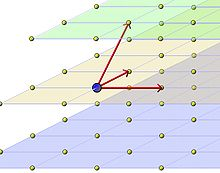
\includegraphics[width=5cm]{reseau.jpg}
    \caption{un exemple d'un réseau euclidien de dimension 3 .}
    \label{fig:reseau}
  \end{center}
  \end{figure}
Dans un réseau, des problèmes naturels se posent, comme la recherche d’un vecteur court, ou la recherche du point le plus proche d’un point donné: \newline
\textit{Définition :} \textbf{Shortest Vector Problem (SVP):}\newline
Etant donné une base $B$ d’un sous réseau $L$ de $Z^n$, trouver un vecteur non nul de $L$ le plus court possible pour la norme euclidienne.\newline
\newline
\newline
\begin{figure}[h!]\begin{center}
    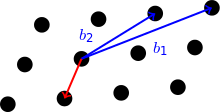
\includegraphics[width=5cm]{svp.png}
    \caption{En bleu la base donnée du réseau, en rouge le vecteur le plus court.}
    \label{fig:svp}
  \end{center}
  \end{figure}
  \newpage
\textit{Définition} \textbf{Closest Vector Problem (CVP):}\newline
Etant donné une base $B$ d’un réseau $L$ de $Z^n$ et un vecteur $v \in Q^n$ , trouver le vecteur de $L$ le plus proche de $v$ pour la norme euclidienne.\newline
\newline
\newline
\begin{figure}[h!]\begin{center}
    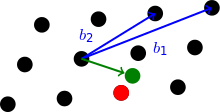
\includegraphics[width=5cm]{cvp.png}
    \caption{En bleu la base donnée du réseau, en vert le vecteur donné,en rouge le vecteur le plus proche du vecteur vert appartenant au réseau.}
    \label{fig:cvp}
  \end{center}
  \end{figure}

Pour ces deux problèmes, trouver la solution est en général difficile sauf si l’on dispose d’une "bonne" base, c’est à dire une base "assez" courte et "assez" orthogonale. La difficulté du problème SVP permet de s’assurer que la clé privée ne peut pas être trouvée facilement. Quant au problème CVP, sa difficulté permet de s’assurer que le bruit d’un chiffré n’est pas calculable donc qu’il est difficile de trouver le texte clair correspondant.\newline
Ainsi Gentry propose le schéma suivant :\newline
\vspace{100\baselineskip}
\newcommand{\bigslant}[2]{{\raisebox{.2em}{$#1$}\left/\raisebox{-.2em}{$#2$}\right.}}
\newline
\textbf{Gentry.KeyGen($\lambda$) :}\newline soit $R$ un anneau : $R$ = $\bigslant{\pmb{\mathbb{Z}}[X]}{f(x)}$, avec $f(x)$ un polynome unitaire de degré $n$ irredictible, soit $I$ un idéal dans $R$, c'est à dire un réseau $I\,\subset\,Z^n$ avec la donnée d'une base $B_I$ : $\bigslant{\pmb{\mathbb{Z}}^n}{B_I} = P(B_I) =\{P_i\}$ est l’espace des textes clairs,avec $P(B_I)$ le parallélépipède associé à cet espace.
Chaque entité choisit un idéal $J$ avec la contrainte $I + J = R$, ainsi que 2 bases $B^{S_k}_J$ (bonne base), $B^{P_k}_J$ (mauvaise base).
Soit $D$ une distribution donnée ajoutant du bruit au texte clair donné.\newline
Soit $p(B^{S_k}_J) = \{\sum_{i=1}^{n}x_ib_i, x_i\in[-1/2, 1/2]\}$ l’ensemble des points du réseau contenus dans le parallélépipède défini par la base $B^{Sk}_J$ et centré à l’origine.\newline
La clé publique est $R$,$B_I$,$B^{Pk}_J$ et la clé privée est $B^{Sk}_J$ .\newline
\textbf{Gentry.Encrypt($R$,$B_I$,$B^{Pk}_J$,$\Pi$) :}\newline
Soit $\Pi$ le message clair à chiffrer.
On lui ajoute du bruit $i$ selon la distribution $D$ $\; : \; \Pi + i \leftarrow \Pi$.\newline
Le chiffré est : $\psi \leftarrow ( \Pi + i  )\; mod\; B^{Pk}_J$\newline
(on soustrait itérativement à $\Pi + i$  des vecteurs de la base $B^{Pk}_J$ jusqu’à ce que le résultat soit dans le parallélépipède $P(B^{Pk}_J))$.\newline
\textbf{Gentry.Decrypt($B^{Sk}_J,\psi$):}
     
Après les travaux de Gentry en 2009, quelques cryptosystèmes ont vu le jour s’inspirant de celui d’origine basé sur les réseaux euclidiens.\newline
\textbf{Le cryptosystème Brakerski-Gentry-Vaikunthanathan (BGV)}\newline
Le cryptosystème BGV pour Zvika Brakerski, Craig Gentry et Vinod Vaikuntanathan consiste en une redéfinition du système de Gentry en
utilisant d’autres problèmes : Decisional Learning With Error (dLWE), Decisional Ring Learning With Error (dRLWE) et Decisional General Learning With Error (dGLWE). C’est ce schéma qui est implementé dans HElib(avec pas mal d’améliorations aujourd’hui).\newline
\newline
\textbf{\textit{BGV.KeyGen($\lambda$,$\mu$)}}\newline
choisir un modul $q$ de taille $\lambda$ bits et choisir les autres paramètres ($d=d(\lambda,\mu,b),\quad n=n(\lambda,\mu,b), \quad N = \lceil(2n+1)log(q)\rceil, \chi = \chi(\lambda,\mu,b))$.\newline
de manière à ce que le schéma soit basé sur une instance de GLWE fournissant $\lambda$ bits de sécurité contre les attaques connues.\newline
Soit $R = \bigslant{\pmb{\mathbb{Z}}[X]}{(x^{d}+1)}$ et noter $params= (q,d,n,N,\chi).$\newline
Tirer $s^{'}\xleftarrow{}{} \chi^{n}$ et fixer $sk = s\xleftarrow{}{}(1,s^{'}_1,.........,s^{'}_n)\in R^{n+1}_q$, la clé privée est $sk$.\newline
Générer une matrice $A^{'}\xleftarrow{}{}R^{N\times m}_q$ uniformément et un vecteur $e \xleftarrow{}{} \chi^{n}$ et fixer $j \xleftarrow{}{}A^{'}s^{'} + 2e$ Soit $A$ la matrice de $( n + 1)$ colonnes telle que la première soit $j$ et le reste soit les $n$ colonnes de $-A^{'}$
La clé publique est $pk = A$.\newline
\newline
\textbf{\textit{BGV.Encrypt($params,pk,m$)}.}\newline
Pour chiffrer un message $m \in R_2$, fixer $m^{'}\xleftarrow{}{}(m,0,.........,0)\in R^{n+1}_q$, tirer $r\xleftarrow{}{} R^N_2$ et retourner le chiffré $c \xleftarrow{}{} m^{'}+A^Tr\in R^{n+1}_q.$\newline
\newline
\textbf{\textit{BGV.Decrypt($params,sk,c$)}.}\newline
Retourner $m \xleftarrow{}{} (\;\langle c,s\rangle \;mod\;q)\;mod \;2$
\newpage
\textbf{Le cryptosystème de Fan et Vercautreen (FV)}\newline
\begin{table}[h!]
  \centering
  \caption{tableau récapitulatif des variables utilisées dans le schéma de FV }
  \label{tab:recapitulatif_des_variables}
  \begin{tabular}{|c|l|}
    \hline
    $q$ &coefficient modulaire dans l'éspace de messages clairs clair \\
    \hline
    $t$ & coefficient modulaire dans l'éspace de messages chiffrés\\
    \hline
    $n$ & une puissance de 2\\
    \hline
    $(x^{n}+1)$ & polynôme de degré n\\
    \hline
    $R$ & l'anneau $\bigslant{\pmb{\mathbb{Z}}[X]}{(x^{n}+1)}$\\
    \hline
    $R_a$ & l'anneau $\bigslant{\pmb{\mathbb{Z_a}}[X]}{(x^{n}+1)}$ avec des coefficients reduit modulo a\\
    \hline
    $w$ & base dans laquel les éléments de messages chiffré sont décompsé durant la rélinearisation\\
    \hline
    $\lambda$ & paramètre de sécurité\\
    \hline
    $\Delta$ & le quotient $\lfloor\dfrac{q}{t}\rfloor$\\
    \hline
    $pk$ & la clé publique\\
    \hline
    $sk$ & la clé secrète\\
    \hline
    \end{tabular}
  \end{table}


\paragraph{ Espace de texte clair .}

L'espace de message clair est $R_t$ c'est-à-dire des polynômes de degré inférieur à $n$ avec des coefficients modulo $t$. On utilise également la structure de l'anneau $R_t$, par exemple, un produit de deux polynômes en texte clair deviennent le produit de deux polynômes avec $x^n = -1$.\newline
Si on veut chiffrer une information on doit passer par un processus d'encodage, par exemple, si on veut chiffrer un entier ce dernier doit être transformer en un polynôme de $R_t$. Le processus d'encodage et de décodage sera détaillé plus tard.\newline 
\paragraph{ Espace de texte chiffré .}
Les messages chiffrés dans le schéma de FV ces sont des vecteurs  des polynomés de taille au mois égale a deux, et qui grandissent en taille avec la multiplication et qui va étre détailler au moment de présenter le processus de chiffrement. 
\textit{Algorithme}
Le schéma de Fan et Vercautreen contient sept algorithmes : \newline

 \begin{description}
 \item[SecretKeyGen$(\lambda)$:]  on choisit aléatoirement s dans $R_2$ et on prend $sk=s$.
 \item[PublicKeyGen$(sk)$ :] .
 \item[EvaluationKeyGen $(sk, w)$:] $for\quad i\in \{1......l\}$ on choisti $a_i\xleftarrow{}{}R_q$,$e_i\xleftarrow{}{}\chi.$\newline
 $$evk = ([-(a_is+e_i)+w^is^2]_q, a_i)$$
 \item[Encrypt $(pk, m)$:] Pour $m \in R_t$ et $Pk = (p_0, p_1)$ échantillonner, $u\xleftarrow{}{} {R_2}$, et $e_1,e_2 \xleftarrow{}{} \chi$.
 \newline et on calcul $Enc(m) = ct = ([\Delta m + p_0 u + e_1]_q, [p_1 u + e_2]_q).$
 \item[Decrypt $(sk, ct)$:] on a $s = sk $, soit $c_0 = ct[0]\quad et\quad c_1 = ct[1]$, on a $Dec(ct) = [\lfloor\dfrac{t}{q}[c_0 + c_1 s]_q\rceil]_t$
 \item[Add  $(ct_0, ct_1)$:]  $ct_0 + ct_1 = (ct_0[0] + ct_1[0], ct_0[1] + ct_1[1])$.
 \item[Multiply $(ct_0, ct_1)$:] on clacul, \newline
 $$c_0 = [\lfloor\dfrac{t}{q}ct_0[0]ct_1[0]\rceil]_q.$$
 $$c_1 = [\lfloor\dfrac{t}{q}(ct_0[0]ct_1[1] + ct_0[1]ct_1[0])\rceil]_q.$$
 $$c_2 = [\lfloor\dfrac{t}{q}ct_0[1]ct_1[1]\rceil]_q .$$ 
 aprés on exprime $c_2 $ dans la base $w$ $$c_2 = \sum_{i=1}^{l}c_2^{(i)}w^i.$$
 $$c_0^{'} = c_0 + \sum_{i=1}^{l}evk[i][0]c_2^{(i)} .$$
 $$c_1^{'} = c_1 + \sum_{i=1}^{l}evk[i][1]c_2^{(i)} .$$
 et donc le produit de deux chifrés sera $(c_0^{'}, c_1^{'}).$
  \end{description}
\subsection{Apprentissage automatique}
\subsubsection{Définition}
L'apprentissage automatique (machine learning en anglais) est une discipline consacrée à l'analyse des données. cette discipline nous permet de créer des connaissances automatiques à partir des données brutes, cela consciste à la mise en place des algorithmes (ou modèle) qui vont etre exploiter pour prendre des décisions.\newline
Le schéma suivant montre le mode de fonctionnement d'un modèle en machine learning.\newline
\begin{figure}[h!]\begin{center}
    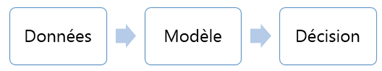
\includegraphics[width=5cm]{m_learning.png}
    \caption{mode de fonctionnement d'un modèle en machine learning}
    \label{fig:m_learning}
  \end{center}
  \end{figure}

  \begin{enumerate}
 \item a partir des données on construit le modèle.
 \item Le modèle permet de prendre des décisions.
 \item On se sert du modèle sur de nouvelles données afin de prendre des décisions.
 \end{enumerate}
\subsubsection{Les données}
Les données sont appelées échantillons, en machine learning ils sont souvent présenter sous fourme des vecteurs.\newline
$x=(x_1, x_2,.............,x_p).$\newline
où $p$ est le nombre de coordonnées aussi appelé nombre d’attributs.\newline
En machine learning on a deux types des données :\newline
\newline
\textbf{Les données labélisées :} on donne à l’algorithme un certain nombre d’exemples sur lesquels l'algorithme  apprend, et ces exemples sont « labellisés », c’est-à-dire qu’on leur associe un résultat désiré . L’algorithme a alors pour tâche de trouver la loi qui permet de trouver la sortie en fonction des entrées.\newline
\newline 
\textbf{Les données non-labellisée :} définition2.
\subsubsection{La décision} 
On distingue deux types des décisions pour les algorithmes en machine learning. \newline
\textbf{Sorties catégorisées ou discrètes :} le nombre de sorties possible est fini. Dans ce cas, les sorties possibles sont appelées classes\newline
\textbf{Sorties non-catégorisées ou continues :} le nombre de sorties possible est infini dont la sortie de l'algorithme y est dans $R$ .\newline
\begin{figure}[h!]\begin{center}
    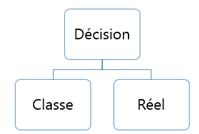
\includegraphics[width=5cm]{classifictation_vs_regression.png}
    \caption{En bleu la base donnée du réseau, en vert le vecteur donné,en rouge le vecteur le plus proche du vecteur vert appartenant au réseau.}
    \label{fig:cvp}
  \end{center}
  \end{figure}

\hspace*{5cm}{}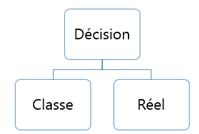
\includegraphics[scale=1]{classifictation_vs_regression.png}
\subsubsection{Types d'apprentissages}
il y a deux pricipaux systèmes d'apprentissage qui définissent les différents modes de fonctionnement de machine learning.\newline
\title{\textbf{L’apprentissage supervisé ou analyse discriminatoire}}\newline
L'objectif de la classification supervisée est principalement de définir des règles permettant de classer des objets dans des classes
à partir de variables qualitatives caractérisant ces objets. Les méthodes s'étendent souvent à des variables $Y$ quantitatives (régression).
On dispose au départ d'un échantillon dit d'apprentissage dont les classes sont connu. Cet échantillon est utilisé pour l'apprentissage des règles de classement.\newline 
\title{\textbf{L’apprentissage non-supervisé ou clustering}}\newline
Le clustering consiste à regrouper les données en groupes homogènes appelés classes ou clusters, de sorte que les éléments à l’intérieur d’une même classe soient similaires, et les éléments appartenant à deux classes différentes soient différents.  

\subsection{Quelques Applications de chiffrement homomorphe a l'apprentissage automatique}
Il est devenu possible de déléguer l'exécution d'un algorithme d'apprentissage à un service informatique tout en conservant la confidentialité des données. \newline
Parmis les travaux qui ont vu le jour  :\newline
\textit{Cryptonets \cite{1gilad2016cryptonets} } :  \newline
Dans cette application la phase d'apprentissage a été effectué sur des données clair  afin d'obtenir le modèle qui va servir dans la phase d'inférence, et ce dernier a été éffectué sur des données chiffrées.\newline
Le jeux des données qui a été utilisé pour cette demonstration est MNIST c'est une base de données de chiffres écrits à la main. C'est un jeu de données très utilisé en apprentissage automatique.\newline
Cryptonets a réalisé un taux de réussite de 99 \% et prend 570 secondes pour fournir une réponse par exemple.\newline
\textit{ \cite{dowlin2017manual} } :\newline

\newpage
\newpage
\section{Application}
La deuxième partie de mon stage a été consacré a l'implementation de quelques algorithmes d'apprentissage automatique.\newline
Au début l'implementation s'effectue sur des données clairs pour bien comprendre les différents paramètres qu'il faut prendre en compte pour evaluer la qualité du modèl, et par la suite l'imlementation des memes algorithmes sur des données chiffrées et comparer les résultats obtenu. \newline      
\subsection {Regression Lineaire}
La regression linéaire est une modélisation linéaire qui permet de fournir des prédictions a partir des informations provenant du passé, 
Dans ce modèle on établi une relation entre une ou plusieurs variables explicatives $(x_1,x_2,..........,x_n)$ et une variable expliquée souvent noté par $Y$.\newline
La fonction d'evaluation dans la régression lineaire est la suivante : \newline
$$Y =h_{\theta}(x) = \theta^T = \sum_{i=1}^{n} \theta_ix_i $$\newline
ou $\theta_j (j=1................n)$ ces sont les paramètres du modèl qu'on devra estimer au moyen de techniques statistques parmis  lesquelles on trouve la descente de gradient stochastique.\newline
\subsubsection{Algorithme de descente de gradient stochastique \textit{(stochastic gradient descent)}}.\newline
Cet algorithme permet de minimiser la fonction d'erreur (cost function) qui s'écrit sous la forme : \newline
$$J(\theta) = \dfrac{1}{2m}\sum_{i=1}^{m} (h_{\theta}^{x^{(i)}} - y^{(i)})^2$$\newline  
\newline
La descente de gradient stochastique premet de choisir les paramètres du modèl $\theta_i$ afin de minimiser la fonction d'erreur.\newline
Algorithme : \newline
\textit{inisialiser :} $\theta_i\quad pour\quad i=1 \quad jusqu'a\quad n$\newline
\textit{inisialiser : }$learning\_rate\quad(\alpha)$\newline
\textit{répéter}\{\newline 
\hspace*{1cm}\textit{pour j=1 jusqu'à m}\{
$$\theta_j := \theta_j - \alpha  \dfrac{1}{m}\sum_{i = 1}^{m} (h_\theta(x^{(i)}) - y^{(i)})x_j^{(i)} \quad(pour\, tout \, j)$$
\hspace*{1cm}\}\newline

\subsection{Regression Logistique}
La regression logistique est une méthode statistique pour analyser un ensemble des données dans lequel il existe une ou plusieurs variables indépendantes qui servent a déterminer un résultat.\newline
L'objectif de la régression logistique est de trouver le meilleur modèle pour décrire le lien entre les vraiables explicatives et la variable dépondante ou la variable expliquée.\newline
Dans ce qui suit, nous noterons $Y$ la variable à prédire (variable expliquée), $X = (X_1, X_2, ..., X_J)$ les variables prédictives (variables explicatives). \newline
Dans le cadre de la régression logistique binaire, la variable $Y$ prend deux modalités possibles \{1, 0\}. Les variables $X_j$ sont exclusivement binaire. \newline
La fonction de prédiction dans la régression logistique est la suivante :\newline
$$h_{w,b}(x)=\dfrac{1}{1 + exp(-w^T x - b)}$$
ou $w_j$ : ces sont les paramètres du modèle.\newline
Pour l'estimation des paramètrs du modèle, on utilise l'algorithme de la descente de gradient stochastique qui sert a minimiser la fonction d'erreur :\newline
$$J(w,b) = \dfrac{1}{m}(\sum_{i=1}^{m}-y^{(i)}log(h_{w,b}(x^{(i)}))-(1-y^{(i)})log(1 - h_{w,b}(x^{(i)}))).$$\newline 
L'implémentation de l'algorithme de la descente de gradient stochastique se fait de la meme façon que la régression linéaire.\newline
\textit{répéter}\{\newline 
\hspace*{1cm}\textit{pour j=1 jusqu'à m}\{
$$w_j := w_j - \alpha  \dfrac{1}{m}\sum_{i = 1}^{m} (h_{w,b}(x^{(i)}) - y^{(i)})x_j^{(i)} \quad(pour\, tout \, j)$$
$$ b := b - \alpha  \dfrac{1}{m}\sum_{i = 1}^{m} (h_{w,b}(x^{(i)}) - y^{(i)})$$
\hspace*{1cm}\}\newline
\} 
\subsection{SEAL:Simple Encrypted Arithmetic Library}
\subsubsection{Présentation de la bibliothèque}
SEAL est une bibliothèque de chiffrement homomorphe qui est en cours de developpement par des chercheurs en cryptographie a microsoft elle fait partie de logiciel libre, elle est écrit en C++11.
Un manuel détaillé pour l'utilisation de la version la plus récente de SEAL est disponible sur le lien \url{https://www.microsoft.com/en-us/research/publication/simple-encrypted-arithmetic-library-seal-v2-2/}. \newline
 \newline
\textbf{différence entre l'implémentation de SEAL et cryptosysteme Fan et Vercautreen}  \newline
Dans SEAL, certaines opérations sont implémentées d'une facon différente qui est plus générale par rapport au cryptosystème FV.\newline
Dans cette partie on traite cette différence en détail.\newline
\textbf{\textit{message chiffré$(Ciphertext)$, message clair$(plaintext)$ dans SEAL.}}\newline
Les messages clairs dans SEAL c'est sont des élément de $R_t$ comme dans le cryptosysème Fan et Vercautreen,
Dans la version 2.2 les messages clairs sont présenter dans une classe Plaintext .\newline
Pour clarifier la généralisation des opérations FV, les messages chiffrés sont des vecteurs de taille qualconque et chaque composant chiffré correspond à une puissance de la clé secrète, Si on suppose que $ct = (c_0,..........,c_k)$ est un message chifré de taille $k+1$ alors,\newline
$c_0\quad correspond\quad à\quad s^0.$\newline
$c_1\quad correspond\quad à\quad s^1.$\newline
$c_k\quad correspond\quad à\quad s^k.$
\newline
 Dans SEAL les messages chiffré sont présenter dans une classe Ciphertext.\newline
 \textbf{Déchiffrement d'un message de taille quelconque.}\newline
soit $ct = (c_0, c_1, .........., c_k)$ une message chiffré de taille $k+1.$\newline
$Dec(ct) = Dec((c_0, c_1, .........., c_k)) = [\lfloor\dfrac{t}{q}[ct(s)]_q\rceil]_t = [\lfloor\dfrac{t}{q}[c_0 + c_1s+c_2s^2+.......,c_ks^k]_q\rceil]_t$\newline
Multiplication et addition de deux message dans SEAL\newline
\textit{Addition:}\newline
soient $ct_1$ et $ct_2$ deux message chifré telque,\newline
$ct_1 = (c_0,............,c_j)$, $ct_2 = (d_0,............,d_k)$
\newline
\textit{Addition : }\newline
\newline
$si\quad on\quad suppose\quad que\quad k\quad \leq \quad j\quad on\quad a \quad:$\newline
\newline
$Add(ct_1, ct_2) = (ct_1[0]+ct_2[0],ct_1[1]+ct_2[1],..............,ct_1[k]+ct_2[k])$\newline
\newline
\textit{Multiplication:}\newline
\newline
$Mult(ct_1, ct_2) = (C_1,C_2,............., C_{j+k})$ avec :\newline
$$C_m = [\lfloor\dfrac{t}{q}(\sum_{r+s=m}^{}c_rd_s)\rceil]_q.$$
\textit{Relinearization:}\newline
\newline
\textit{Autres opérations définies dans SEAL:}\newline
Toutes les opérations sont définies dans une classe Evaluator\newline
\begin{description}
 \item[Evaluator::negate :] permet d'evaluer la negation homomorphiquement,
 \item[Evaluator::add\_plain :] permet d'additioner Plaintext a un Ciphertext,
 \item[Evaluator::multiply\_plain :] multiplication entre Plaintext et Ciphertext,
 \item[Evaluator::sub\_plain :] soustraction entre Ciphertext et Plaintext,
 \item[Evaluator::multiply\_many :] multiplicatioon de plusieurs Ciphertext,
 \item[Evaluator::add\_many :] addition de plusieurs Ciphertext,
 \item[Evaluator::square :] elevation puissance 2,
 \item[Evaluator::exponentiate :] Elévation d'un message chiffré à une puissance qui est un nombre entier,
  \end{description}
  \subsection{Régression linéaire et chiffrément homomorphe}
  \subsubsection{Implémentation de stochastic gradient descent \cite{codehomomorphicencryptionlr}}
  Dans cette partie le travail demandé est d'implémenter l'algorithme cité dans la partie $4.1$ avec des données chiffrées en utilisant les fonctions de chiffrément homomorphe définie dans SEAL. \newline 
  Le but de cette implementation est d'évaluer la performance du modèle obtenu a partir des données chiffrées et de le comparer au niveau des différents paramètres avec le modèle obtenu a partir des données clairs.\newline
  Parmis les paramaètres qu'il faut prendre en compte pour évaluer l'éfficacité d'un modèle en machine learning c'est la fonction d'erreur(loss en anglais).\newline  
  \subsubsection{Problèmes}
  Parmis les problèmes que j'ai rencontré pendant l'implementation de l'algorithme  sur les données chiffrées c'est qu'on un paramètre associé a chaque texte chiffrées pendant sa création (budget de noise), au début il est initialisé selon le paramètres qu'on choisit pour notre cryptosystème  et après chaque opération sur le texte chiffré la valeur diminue et quand il atteint la valeur 0 le texte chiffré devient indéchiffrable donc la solution est de savoir controler ce paramètre.
  \subsubsection{Solution}
  La solution pour ce probème comme il le montre la figure suivante :\newline
  \begin{figure}[h!]\begin{center}
    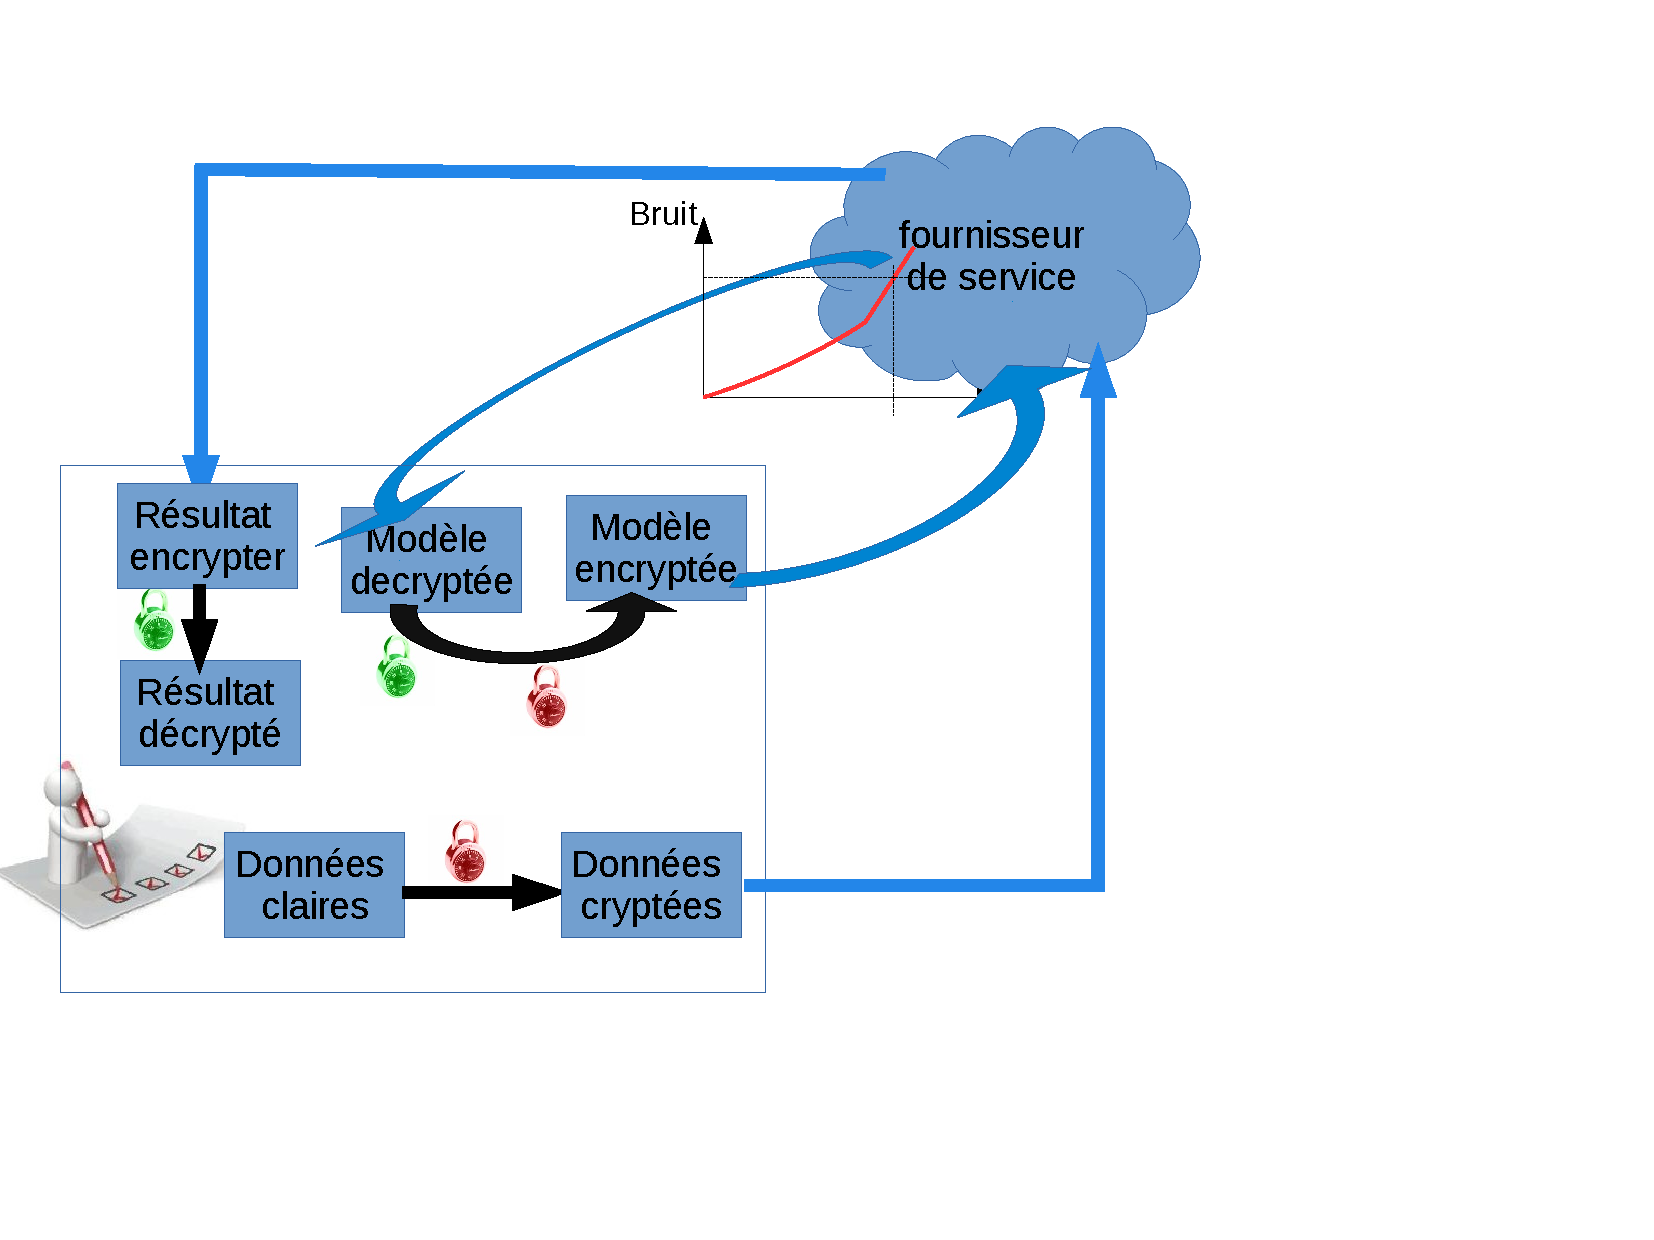
\includegraphics[width=10cm]{SchemaM.pdf}
    \caption{Mode de fonctionnement de modèle avec des données chiffrées}

    \label{fig:loss_linear}
  \end{center}
  \end{figure}
  \newline
 L'idée c'est qu'après un nombre d'itération précis dans l'algorithme de la descente de gradient stochastique on renvoit le modèle qui est l'élément sur lequel on efectue le plus d'opérations, c'est qui signifie que le budget de noise diminue constamment, a la personne qui détient la clé secrète pour qu'il déchiffre et rechiffre et avec cette méthode on repart avec un budget de noise élevé.

  \subsubsection{Résultats obtenu et comparaison}
  On voit bien sur la figure 5 qu'après 613 itérations ( l'execution de l'algorithme a pris presque 18 heures ) la variation de la fonction d'erreur dans le deux cas est presque similaire.  
  \begin{figure}[h!]\begin{center}
    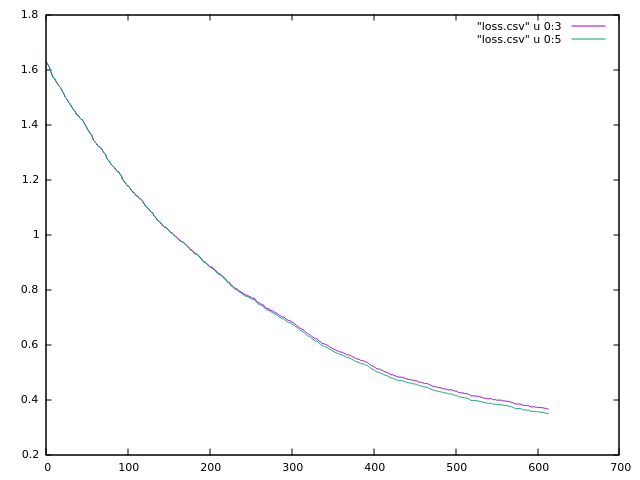
\includegraphics[width=10cm]{loss_linear_regression.png}
    \caption{En vert la variation de la fonction d'erreur sur les données clairs\newline
            En mauve la variation de la fonction d'erreur sur les données chiffrées}

    \label{fig:loss_linear}
  \end{center}
  \end{figure}
\newpage
  \subsection{Régression logistique et chiffrement homomorphe}
  \subsubsection{Implementation de stochastic gradient descent}
  Dans cette partie le travail demandé est d'implementer l'algorithme cité dans la partie $4.2$, cette partie est similaire au niveau implementation que celle de la régression linéaire sauf que cette fois on a la fonction sigmoid a la place de la fonction linéaire.
  et comme dans la fonction sigmoid on a le terme exponentielle qui n'est pas définie dans SEAL il a fallu approximer avec d'autres fonctions.\newline
  \textit{Première tentative}\newline
  La prémière idée est d'approximmer la fonction sigmoid avec un développement de taylor comme a été introduit dans l'application "Manual for using homomorphic encrytpion for bioinformatics",\newline    
  \newcommand\omicron{o}
  $$\dfrac{1}{1+e^{-x}} = \dfrac{1}{2} + \dfrac{1}{4}x - \dfrac{1}{48}x^3 + \dfrac{1}{480}x^5 - \dfrac{1}{80640}x^7 + \omicron(x^9)$$
  Avec cette approximation la fonction exponentiate qui calcul la puissance d'un réel dans SEAL ne permet pas de traiter des messages chiffrés qui n'ont pas un budget de noise assez grand . donc le message apres l'application de la fonction exponentiate devient indéchifrable.\newline
  cette idée n'a pas abouti donc il a été demandé de chercher une autre approximation.\newline  
  \textit{Deuxième tentative}\newline  
  La deuxième approximation c'était avec la fonction piecewise qui est défini de la façon suivante :\newline
  \begin{equation}
f(x)=
\left\lbrace
\begin{array}{ccc}
0  & \mbox{si} & x<-2\\
1/2 + x/4 & \mbox{si} & -2<x<2\\
1 & \mbox{si} & x>2
\end{array}\right.
\end{equation} 
Avec cette approximation il a fallu décrypter la valeur de x vu que dans SEAL on a pas des opérateurs pour comparer deux messages chiffrés.\newline
  \subsubsection{Résultats obtenu et comparaison}
  \begin{figure}[h!]\begin{center}
    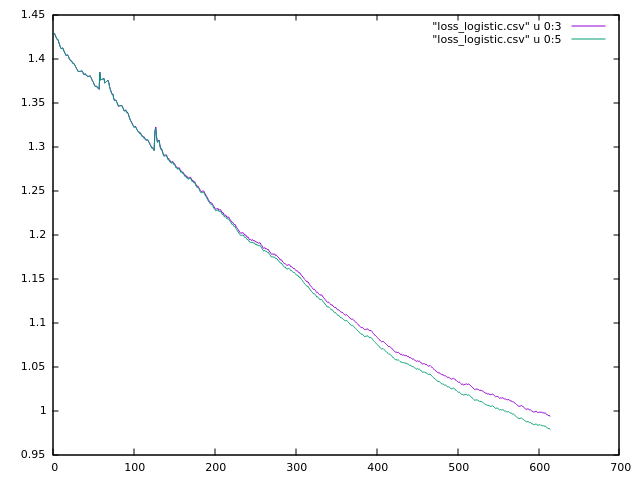
\includegraphics[width=10cm]{loss_logistic_regression.png}
    \caption{En vert la variation de la fonction d'erreur sur les données clairs\newline
            En mauve la variation de la fonction d'erreur sur les données chiffrées}
     \label{fig:loss_logistic}
  \end{center}
  \end{figure}
\newpage
\bibliographystyle{unsrt}
\bibliography{/home/benissa/Bureau/rapport-de-stage/biblio-rapport.bib}
\end{document}
